%==============================================================================
\chapter{De moleculaire oorsprong van chemische energie}
%==============================================================================

\section{De oorsprong van chemische energie}

In het vorige hoofdstuk hebben we de eerste wet van de thermodynamica ontwikkeld als een krachtig hulpmiddel om  de energieverandering in fysische en chemische processen te beschrijven. De thermodynamica vertelt ons \emph{hoeveel} energie tijdens een proces vrijkomt of wordt opgenomen, maar zij verklaart niet \emph{waarom} verschillende stoffen überhaupt een verschillende energie bezitten. Waarom komt bij de reactie van waterstof met zuurstof zoveel energie vrij? Waarom is energie nodig om water opnieuw te ontleden? Waarom is grafiet onder normale omstandigheden stabieler dan diamant, hoewel beide uitsluitend uit koolstofatomen bestaan?

De antwoorden op deze vragen kunnen niet worden gevonden door uitsluitend naar de stof als geheel te kijken. Zij liggen verborgen op een veel kleinere schaal, namelijk in de opbouw van de atomen waaruit de stof bestaat. Uiteindelijk worden alle chemische eigenschappen bepaald door de elektronen rond de atoomkernen en door de manier waarop deze elektronen chemische bindingen vormen.

De oorsprong van chemische energie ligt dus in de elektronische structuur van atomen en moleculen. Om dit te begrijpen moeten we afdalen naar de microscopische wereld van de materie. Dat betekent echter niet dat we een volledige cursus kwantummechanica zullen ontwikkelen. Het doel van dit hoofdstuk is veel bescheidener, maar tegelijk veel relevanter: we willen begrijpen welke fundamentele idee\"en aan de basis liggen van de moderne beschrijving van atomen en hoe deze uiteindelijk leiden tot chemische bindingen en de energieverschillen die we in de thermodynamica beschrijven.

\section{Van de klassieke fysica naar de kwantummechanica}

Vandaag lijkt het vanzelfsprekend dat alle materie is opgebouwd uit stabiele atomen. Aan het begin van de twintigste eeuw was dit echter allesbehalve vanzelfsprekend.

Volgens de klassieke natuurkunde zou een elektron nooit langdurig rond een atoomkern kunnen bewegen. Een elektron bezit immers een elektrische lading. Wanneer een geladen deeltje een kromme baan volgt, ondergaat het voortdurend een versnelling. Volgens de elektromagnetische theorie van Maxwell zendt een versnellende elektrische lading elektromagnetische straling uit en verliest zij daarbij energie. De gevolgen hiervan zijn verstrekkend: indien een elektron voortdurend energie verliest, zal zijn baan steeds kleiner worden totdat het uiteindelijk op de atoomkern terechtkomt. De klassieke natuurkunde voorspelt dus dat stabiele atomen helemaal niet kunnen bestaan.

Er ontbreekt dus iets fundamenteels in de klassieke beschrijving van de natuur. De vraag die natuurkundigen zich moesten stellen was verrassend eenvoudig: wat als elektronen zich niet gedragen zoals de klassieke mechanica voorspelt? Gedurende meer dan twee eeuwen vormde de klassieke mechanica van Newton de basis van vrijwel alle natuurkundige berekeningen. Tegen het einde van de negentiende eeuw leek het alsof de natuurkunde vrijwel voltooid was. Juist op dat ogenblik begonnen echter experimenten te verschijnen die zich niet langer door de klassieke theorie lieten verklaren. De instabiliteit van het atoom vormde \'e\'en van de eerste aanwijzingen, maar zeker niet de enige. Ook de straling die door warme voorwerpen wordt uitgezonden, het foto-elektrisch effect en de karakteristieke spectra van atomen bleken fundamenteel af te wijken van de voorspellingen van de klassieke fysica.

Gaandeweg werd duidelijk dat de klassieke natuurkunde niet fout was, maar een benadering vormde die uitstekend werkt voor macroscopische objecten. Op de schaal van atomen en elektronen gelden echter andere natuurwetten. Om de structuur van materie te begrijpen was daarom een volledig nieuwe theorie noodzakelijk. Deze theorie kreeg de naam \emph{kwantummechanica}.

\section{Energie als discrete grootheid}

Aan het einde van de negentiende eeuw leek de klassieke natuurkunde vrijwel voltooid. De bewegingswetten van Newton, de thermodynamica en de elektromagnetische theorie van Maxwell konden een groot aantal natuurkundige verschijnselen succesvol beschrijven. Toch bleef één hardnekkig probleem onopgelost: de straling die wordt uitgezonden door een warm voorwerp.

Iedereen heeft dit verschijnsel al waargenomen. Een metalen staaf die wordt verwarmd, begint eerst donkerrood te gloeien. Bij een hogere temperatuur verandert de kleur geleidelijk naar oranje, vervolgens geel en uiteindelijk bijna wit. De kleur van het uitgezonden licht hangt dus rechtstreeks samen met de temperatuur van het voorwerp.

De natuurkundigen van die tijd wilden deze warmtestraling theoretisch beschrijven. Daartoe beschouwden zij een ideaal voorwerp dat alle invallende straling volledig absorbeert en opnieuw uitzendt. Een dergelijk voorwerp wordt een \emph{zwart lichaam} genoemd. Het uitgestraalde spectrum van een zwart lichaam bleek experimenteel zeer nauwkeurig meetbaar en vormde daardoor een ideale test voor de bestaande theorieën.

De klassieke theorie voorspelde echter een fundamenteel verkeerd resultaat. Volgens de wetten van de klassieke elektromagnetica zouden de atomen in een warm voorwerp elektromagnetische golven met alle mogelijke frequenties kunnen uitzenden. Bovendien zou elke mogelijke trillingsmodus gemiddeld dezelfde hoeveelheid energie bevatten, overeenkomstig de equipartitiestelling uit de klassieke statistische mechanica.

Het aantal mogelijke trillingsmodi neemt echter zeer sterk toe naarmate de frequentie groter wordt. De klassieke theorie voorspelde daardoor dat vooral straling met een zeer hoge frequentie, zoals ultraviolet licht, een enorme hoeveelheid energie zou bevatten. Wiskundig leidde de theorie zelfs tot de absurde conclusie dat de totale uitgestraalde energie oneindig groot moest zijn.

Dit resultaat staat bekend als de \emph{ultraviolette catastrofe}, ook wel de Rayleigh-Jeans-catastrofe. De voorspelling was duidelijk in tegenspraak met experimenten. In werkelijkheid neemt de intensiteit van de warmtestraling na een bepaalde frequentie juist sterk af, zodat slechts een beperkte hoeveelheid energie wordt uitgestraald (zie Figuur \ref{fig:UVcatastrophe}).

\begin{figure}[htb]
    \centering
    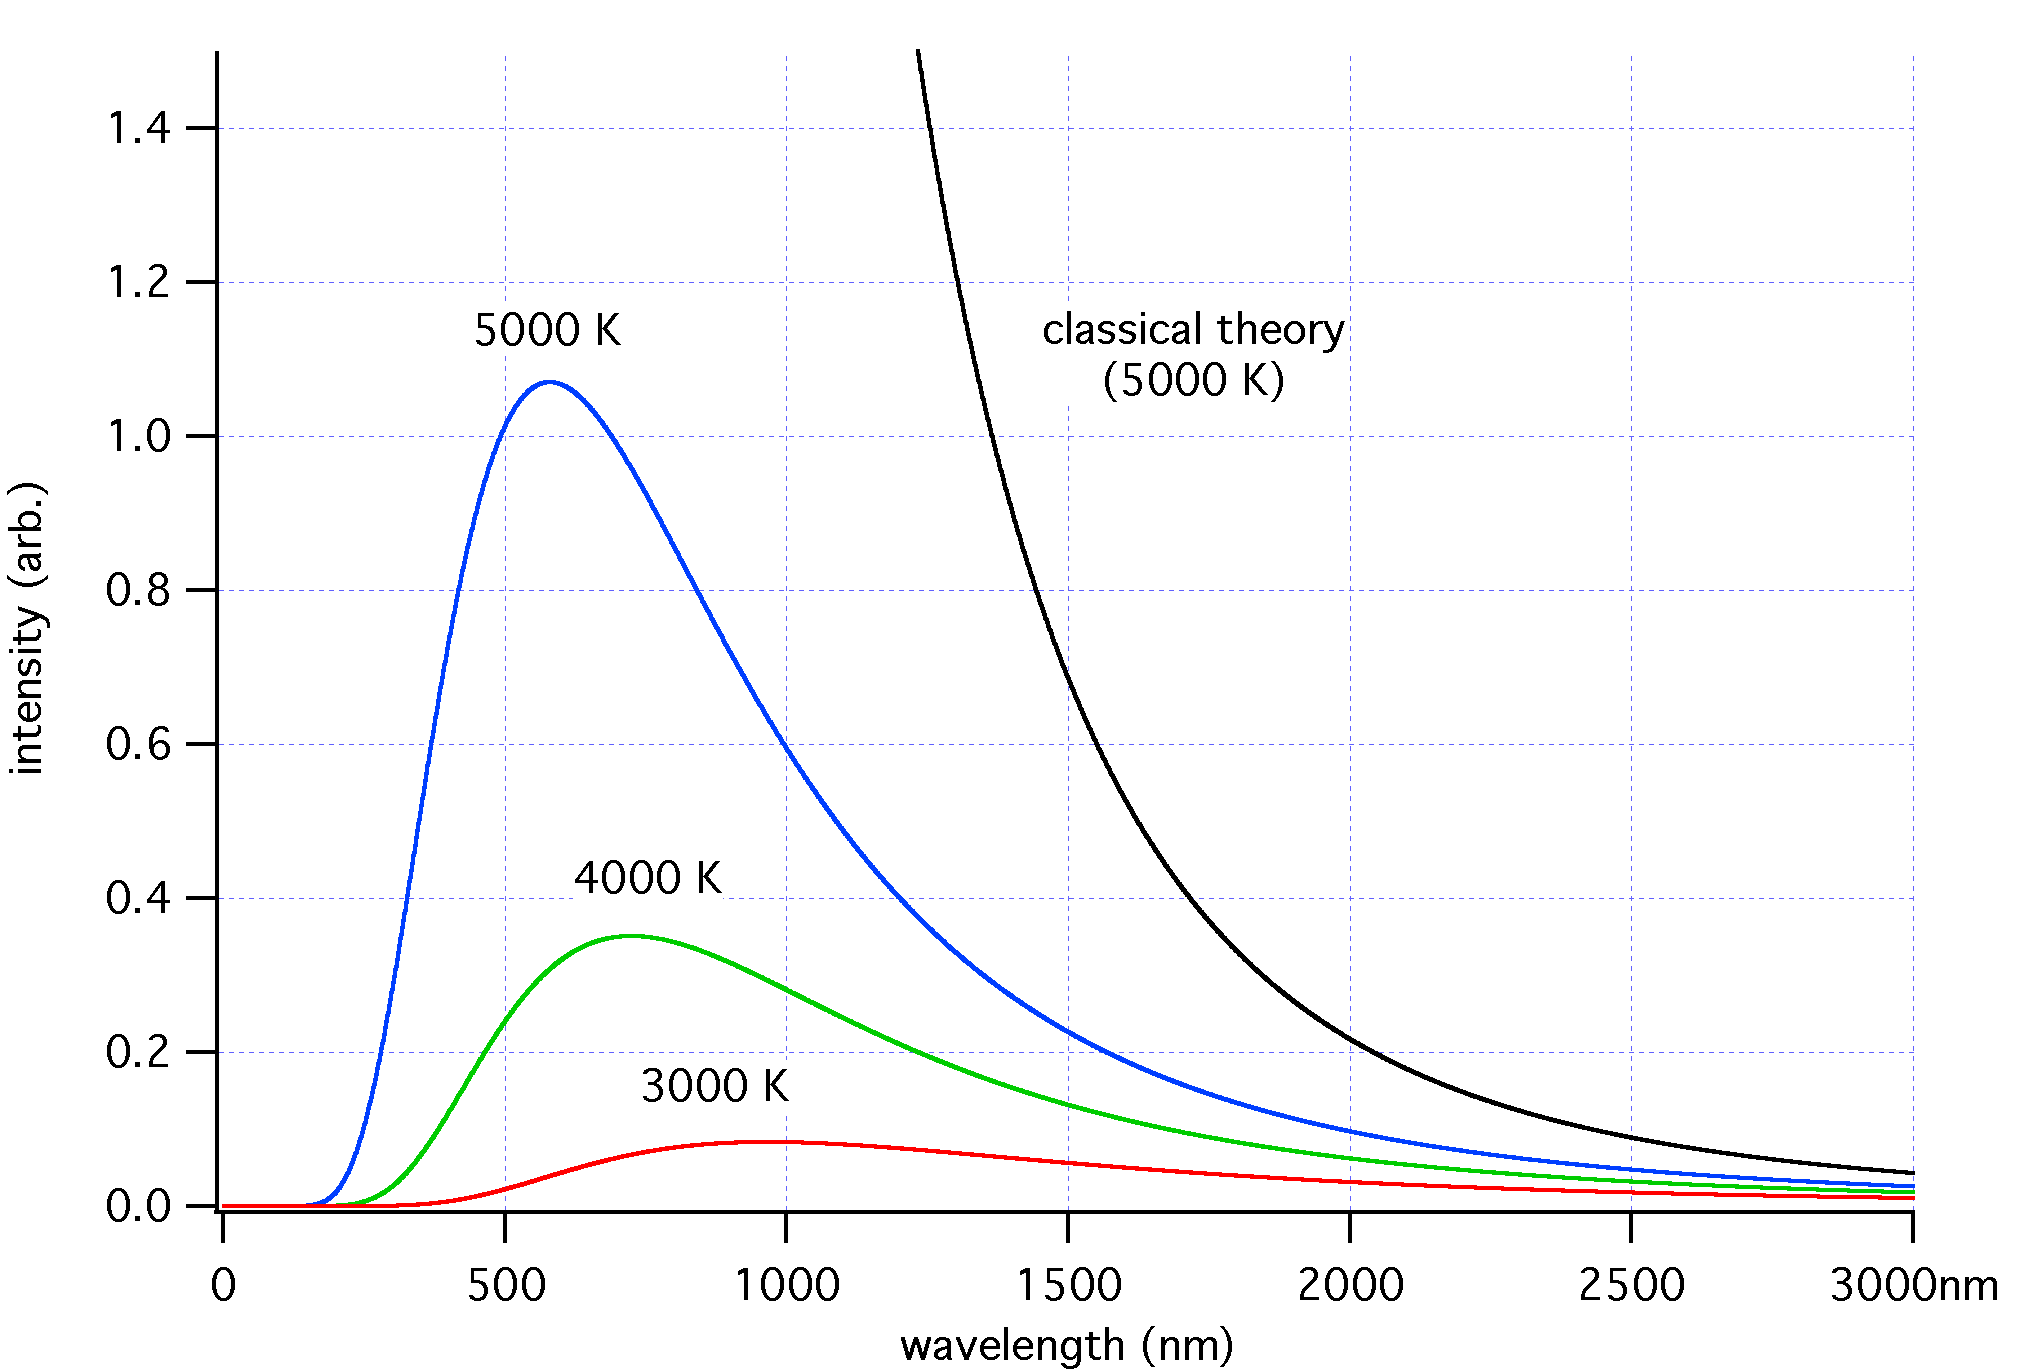
\includegraphics[width=0.8\linewidth]{Afbeeldingen/Blackbody-lg.png}
    \caption{De Ultravioletcatastrofe is de fout bij korte golflengten in de wet van Rayleigh-Jeans voor uitgestraalde energie door een ideaal zwart-lichaam. De fout, die veel meer uitgesproken is voor korte golflengten, is het verschil tussen de zwarte kromme (de verkeerde kromme die wordt voorspeld door de wet van Rayleigh-Jeans) en de blauwe kromme (de correcte kromme die wordt voorspeld door de wet van Planck).}
    \label{fig:UVcatastrophe}
\end{figure}

De vraag was dus fundamenteel: \emph{waarom straalt een warm voorwerp geen oneindige hoeveelheid hoogfrequente straling uit?}  In 1900 stelde de Duitse natuurkundige Max Planck een gedurfde hypothese voor. Hij veronderstelde dat de atomen in een warm voorwerp niet willekeurig energie kunnen opnemen of afgeven. De uitwisseling van energie gebeurt uitsluitend in kleine, ondeelbare pakketjes, die later \emph{kwanta} werden genoemd.

\begin{equation}
\boxed{
E=h\nu
}
\end{equation}
waarin $h$ de constante van Planck is ($h=6.626\times10^{-34}\;\si{\joule\second}$) en $\nu$ de frequentie van de elektromagnetische straling voorstelt.

Deze eenvoudige hypothese had verstrekkende gevolgen. Voor laagfrequente straling is de energie van één quantum klein, zodat vele energietoestanden gemakkelijk bereikbaar zijn. Bij zeer hoge frequenties wordt de energie van één quantum echter veel groter. De trillende deeltjes beschikken dan vaak niet over voldoende energie om een dergelijk quantum uit te zenden. Hierdoor wordt de emissie van hoogfrequente straling automatisch onderdrukt. De experimenteel waargenomen afname van de intensiteit bij hoge frequenties volgde daardoor vanzelf uit Plancks theorie. Zijn vergelijking beschreef het volledige spectrum van de warmtestraling met een nauwkeurigheid die voordien onmogelijk was.

Hoewel Planck zijn hypothese aanvankelijk vooral als een mathematische truc beschouwde, bleek het later een fundamentele eigenschap van de natuur te beschrijven. Voor het eerst werd het klassieke idee verlaten dat energie een volledig continue grootheid is. Op macroscopische schaal zijn de energiekwanta zo klein dat energie continu lijkt te veranderen. Op atomaire schaal worden deze energiestappen echter bepalend voor het gedrag van materie.

\section{Het foto-elektrisch effect}

Hoewel de hypothese van Planck het spectrum van een zwart lichaam perfect kon beschrijven, bleef onduidelijk of de energiekwanta werkelijk een fysische betekenis hadden. Vele natuurkundigen beschouwden de kwantisatie van energie aanvankelijk slechts als een wiskundige truc.

In 1905 gaf Albert Einstein aan Plancks idee een veel diepere betekenis. Hij stelde voor dat licht niet alleen in discrete hoeveelheden wordt uitgezonden of geabsorbeerd, maar dat het zelf uit afzonderlijke energiepakketjes bestaat. Elk van deze pakketjes, later \emph{fotonen} genoemd, bezit dezelfdde gekwantiseerde energie als Planck postuleerde, $E=h\nu$.

Deze hypothese bood een verklaring voor het foto-elektrisch effect, een verschijnsel dat met de klassieke golftheorie van het licht niet kon worden verklaard.

\begin{figure}[htb]
    \centering
    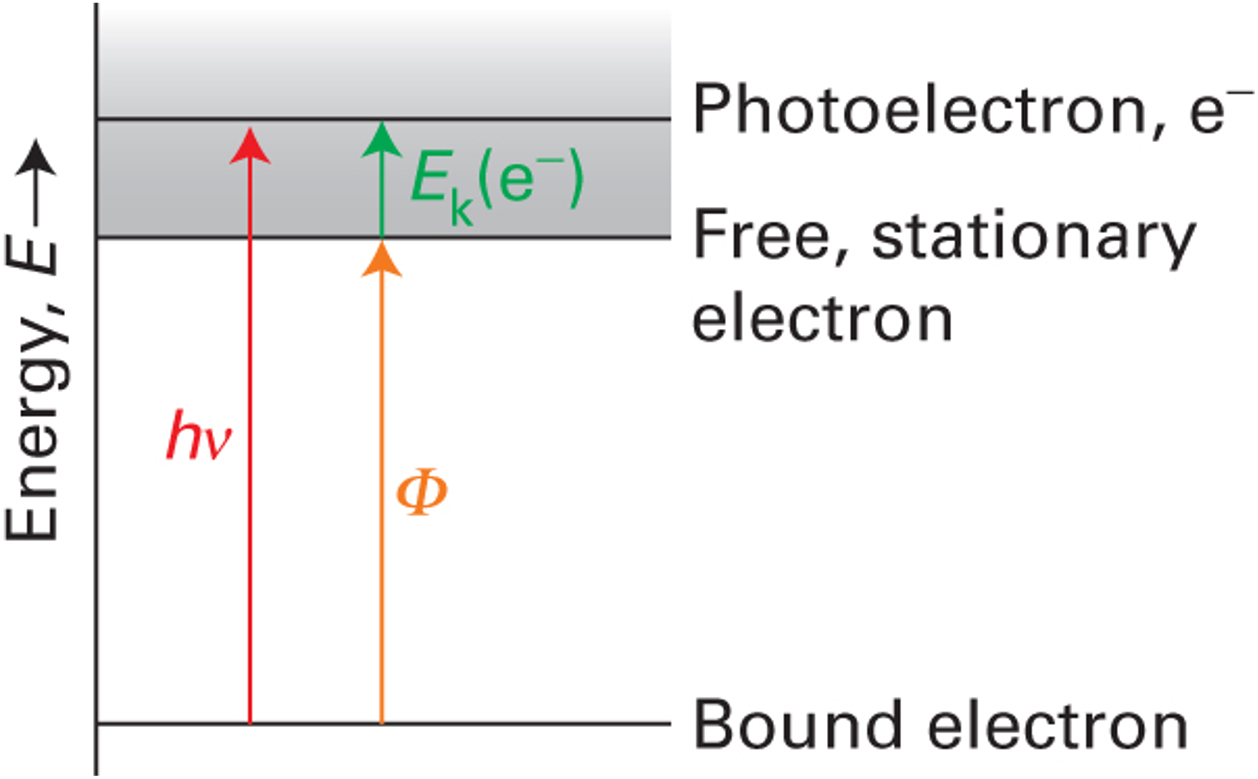
\includegraphics[width=0.5\linewidth]{Afbeeldingen/photoelectric.png}
    \caption{Een invallende elektromagnetische straling met energie $h \nu$ is in staat om een elektron uit het metaal te verwijderen. Hiervoor wordt de energie enerzijds gebruikt om te ontsnappen uit het metaal ($\Phi$) en anderzijds om het elektron te versnellen ($E_k$).}
    \label{fig:photoelectric}
\end{figure}

Wanneer licht op een metalen oppervlak valt, kunnen elektronen uit het metaal worden vrijgemaakt. Klassiek zou men verwachten dat een grotere lichtintensiteit de elektronen steeds meer energie geeft, ongeacht de kleur van het licht. Experimenten tonen echter een volledig ander gedrag.

\begin{enumerate}
\item Onder een bepaalde drempelfrequentie worden helemaal geen elektronen uitgestoten, zelfs niet wanneer de lichtintensiteit zeer groot is.
\item Zodra de frequentie boven deze drempel komt, worden de elektronen vrijwel onmiddellijk vrijgemaakt.
\item De maximale kinetische energie van de uitgestoten elektronen hangt uitsluitend af van de frequentie van het invallende licht en niet van de lichtintensiteit.
\end{enumerate}

Einstein verklaarde deze waarnemingen door aan te nemen dat één elektron telkens slechts één foton absorbeert. Een deel van de energie van dit foton is nodig om het elektron uit het metaal los te maken. Deze minimale energie wordt de \emph{werkfunctie} genoemd en wordt aangeduid met $\Phi$.

Wanneer de energie van het foton groter is dan de werkfunctie, blijft het overschot over als kinetische energie van het uitgestoten elektron. Dit leidt tot de beroemde vergelijking van Einstein (zie Figuur \ref{fig:photoelectric}):

\begin{equation}
h\nu = \Phi + E_{\mathrm{kin,max}}
\end{equation}

of

\begin{equation}
\boxed{
E_{\mathrm{kin,max}} = \frac{1}{2}m_ev^2  = h\nu-\Phi}
\end{equation}

De werkfunctie is een materiaaleigenschap. Typische waarden liggen tussen ongeveer \SI{2}{\electronvolt} - \SI{5}{\electronvolt}, afhankelijk van het gebruikte metaal.

\begin{voorbeeld}{Foto-elektrisch effect}

Een natriumoppervlak heeft een werkfunctie van
$\Phi=\SI{2.30}{eV}$.
Het wordt bestraald met ultraviolet licht met een golflengte van
$\lambda=\SI{250}{nm}$.

De energie van één foton bedraagt

\begin{equation*}
E=\frac{hc}{\lambda}.
\end{equation*}

Invullen geeft

\begin{align*}
E
&=
\frac{(\SI{6.626e-34}{J\,s})
(\SI{3.00e8}{m/s})}
{\SI{250e-9}{m}}
\\
&=
\SI{7.95e-19}{J}
\\
&=
\SI{4.96}{eV}.
\end{align*}

De maximale kinetische energie van het elektron bedraagt bijgevolg

\[
E_{\mathrm{kin,max}}
=
4.96-2.30
=
\SI{2.66}{eV}
\]

Het elektron wordt dus uit het metaal losgemaakt en verlaat het oppervlak met een kinetische energie van \SI{2.66}{eV}.

\end{voorbeeld}

De werkfunctie mag niet worden verward met de ionisatie-energie. De \emph{werkfunctie} is de minimale energie die nodig is om een elektron uit een vast metaal los te maken. Het elektron bevond zich reeds in de geleidingsband van het metaal en hoeft enkel het oppervlak te verlaten. De \emph{ionisatie-energie} is de energie die nodig is om een elektron volledig uit een geïsoleerd atoom of molecuul te verwijderen. Hierbij moet de volledige aantrekkingskracht van de atoomkern worden overwonnen. Omdat een elektron in een metaal reeds relatief vrij kan bewegen, is de werkfunctie doorgaans aanzienlijk kleiner dan de ionisatie-energie van hetzelfde element. Zo bedraagt de werkfunctie van natrium ongeveer \SI{2.3}{eV}, terwijl de eerste ionisatie-energie ongeveer \SI{5.1}{eV} bedraagt.

De verklaring van het foto-elektrisch effect vormde een van de eerste overtuigende bewijzen dat licht zich niet alleen als een golf, maar ook als een verzameling deeltjes kan gedragen. Samen met Plancks hypothese vormde dit het vertrekpunt voor de ontwikkeling van de moderne kwantummechanica.

\section{Het golfkarakter van materie}

Het voorstel van Planck betekende een revolutionaire stap vooruit, maar veranderde aanvankelijk nog niets aan het beeld dat natuurkundigen van materie hadden. Licht werd beschouwd als een elektromagnetische golf, terwijl elektronen en andere materiedeeltjes werden voorgesteld als kleine, duidelijk gelokaliseerde deeltjes.

Dat onderscheid werd al snel minder vanzelfsprekend. Einstein had in 1905 door het foto-elektrisch effect aangetoond dat licht zich in bepaalde omstandigheden ook gedraagt alsof het uit afzonderlijke energiepakketjes bestaat. Licht, dat traditioneel als een golf werd beschouwd, vertoonde dus eveneens een deeltjeskarakter.

In 1924 stelde Louis de Broglie voor dat deze dualiteit ook in de omgekeerde richting moest gelden. Wanneer licht zowel golf- als deeltjeseigenschappen kan vertonen, dan zou materie mogelijk eveneens een golfkarakter bezitten. Hij veronderstelde dat aan ieder deeltje met impuls $p$ een golflengte kan worden toegekend:

\begin{equation}
\boxed{
\lambda=\frac{h}{p}
}
\end{equation}

waarin $h$ de constante van Planck is en $p$ de impuls van het deeltje. Voor een niet-relativistisch deeltje met massa $m$ en snelheid $v$ geldt
\begin{equation}
p=mv
\end{equation}
zodat de de Broglie-golflengte ook kan worden geschreven als
\begin{equation}
\lambda=\frac{h}{mv}.
\end{equation}

De de Broglie-golflengte betekent niet dat een elektron letterlijk als een kleine, materiële golf door de ruimte beweegt. Zij geeft aan dat het gedrag van een deeltje door een golffunctie moet worden beschreven en dat het onder geschikte omstandigheden verschijnselen zoals interferentie en diffractie kan vertonen.

Voor macroscopische voorwerpen is de impuls zo groot dat de bijbehorende golflengte onvoorstelbaar klein wordt. Het golfkarakter is dan experimenteel niet waarneembaar. Voor elektronen op atomaire schaal kan de de Broglie-golflengte daarentegen vergelijkbaar zijn met de afstand tussen atomen. Daardoor kunnen elektronen worden afgebogen door de regelmatige structuur van een kristal, op een vergelijkbare manier als röntgenstraling.

\begin{voorbeeld}{De de Broglie-golflengte van een elektron en een wandelende persoon}

We vergelijken de golflengte van een elektron dat door een elektrisch potentiaalverschil wordt versneld met die van een wandelende persoon.

\bigskip

\textbf{1. Elektron versneld over \SI{150}{\volt}}

Een elektron dat vanuit rust over een potentiaalverschil $U$ wordt versneld, neemt een kinetische energie op gelijk aan

\begin{equation*}
E_{\mathrm{kin}}=eU,
\end{equation*}

waarin $e$ de elementaire lading is. Voor niet-relativistische snelheden geldt eveneens

\begin{equation*}
E_{\mathrm{kin}}= \frac{1}{2}m_ev^2 =\frac{p^2}{2m_e}.
\end{equation*}

De impuls van het elektron kan daarom worden berekend uit

\begin{equation*}
p=\sqrt{2m_e eU}.
\end{equation*}

De de Broglie-golflengte wordt dan

\begin{equation*}
\lambda = \frac{h}{\sqrt{2m_e eU}}.
\end{equation*}

Met
\[
h=\SI{6.626e-34}{\joule\second}, \qquad m_e=\SI{9.109e-31}{\kilogram}, \qquad e=\SI{1.602e-19}{\coulomb}
\]
en
\[
U=\SI{150}{\volt}
\]
volgt
\begin{align*}
\lambda
&=
\frac{\SI{6.626e-34}{\joule\second}}
{\sqrt{
2
(\SI{9.109e-31}{\kilogram})
(\SI{1.602e-19}{\coulomb})
(\SI{150}{\volt})
}}
\\[2mm]
&=
\SI{1.00e-10}{\meter}.
\end{align*}

Bijgevolg is

\begin{equation}
\lambda_{\mathrm{elektron}} \approx \SI{0.100}{\nano\meter}.
\end{equation}

Deze golflengte is van dezelfde orde van grootte als de afstand tussen atomen in een kristal. Elektronen met deze energie kunnen daarom duidelijke diffractiepatronen veroorzaken. Dit vormt een rechtstreeks experimenteel bewijs voor het golfkarakter van materie.

\bigskip

\textbf{2. Een wandelende persoon}

Beschouw vervolgens een persoon met een massa van
\[
m=\SI{75}{\kilogram}
\]
die wandelt met een snelheid van
\[
v=\SI{1.5}{\meter\per\second} = \SI{5.5}{\km\per\hour}
\]
De impuls bedraagt
\begin{equation*}
p=mv
=
(\SI{75}{\kilogram})
(\SI{1.5}{\meter\per\second})
=
\SI{112.5}{\kilogram\meter\per\second}.
\end{equation*}

De bijbehorende de Broglie-golflengte is

\begin{align*}
\lambda
&=
\frac{h}{mv}
\\
&=
\frac{\SI{6.626e-34}{\joule\second}}
{(\SI{75}{\kilogram})(\SI{1.5}{\meter\per\second})}
\\
&=
\SI{5.89e-36}{\meter}.
\end{align*}

Dus

\begin{equation*}
\lambda_{\mathrm{persoon}}
\approx
\SI{5.9e-36}{\meter}
\end{equation*}

Deze golflengte is vele ordes van grootte kleiner dan de afmetingen van een atoom of zelfs van een atoomkern. Het golfkarakter van een wandelende persoon is daarom in de praktijk volledig onwaarneembaar.
\\

De vergelijking toont dat de de Broglie-relatie in principe voor alle materie geldt. Alleen bij deeltjes met een zeer kleine massa en impuls, zoals elektronen, wordt de golflengte groot genoeg om meetbare golfverschijnselen te veroorzaken.

\end{voorbeeld}


\section{De dubbelspleetproef}

De hypothese van De Broglie werd spoedig experimenteel bevestigd. Wanneer een bundel elektronen door een spleet wordt gestuurd, ontstaat op een scherm achter de spleet een patroon dat typisch is voor golven: een afwisseling van heldere en donkere banden. Dit patroon kan alleen worden verklaard wanneer de elektronen zich als golven gedragen.

Wanneer de proef met \'e\'en elektron tegelijk wordt uitgevoerd, verschijnt telkens slechts \'e\'en punt op het scherm. Pas na vele elektronen ontstaat het golfpatroon langzaam. Elk afzonderlijk elektron wordt dus als deeltje gedetecteerd, maar de verdeling van de detectiepunten vertoont een golfkarakter.

\begin{figure}[htb]
    \centering
    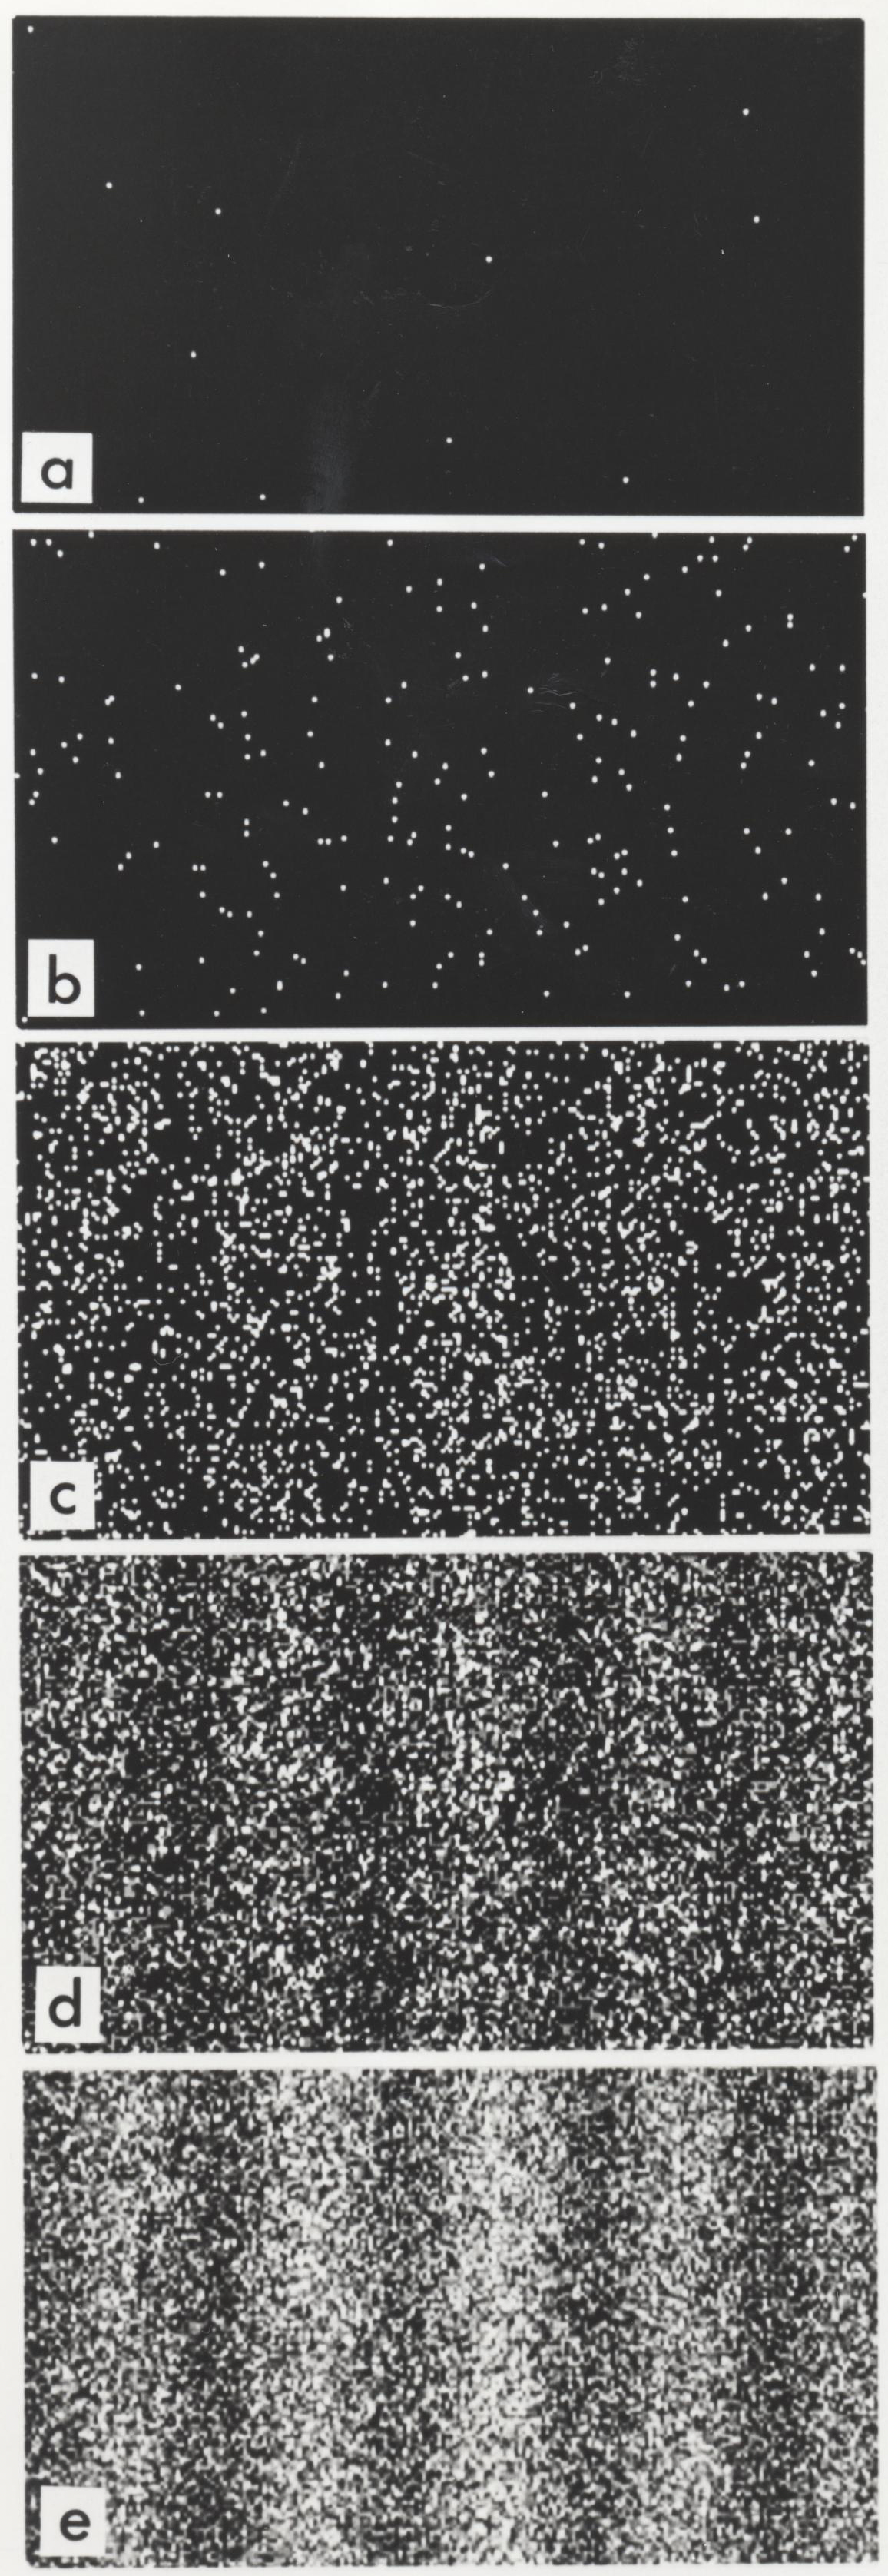
\includegraphics[width=0.3\linewidth]{Afbeeldingen/Double-slit_experiment_results_Tonomura_2.jpg}
    \caption{Resultaten van een dubbelespleetexperiment waaruit de vorming van een interferentiepatroon van afzonderlijke elektronen blijkt. Het aantal elektronen bedraagt 11 (a), 200 (b), 6000 (c), 40000 (d) en 140000 (e).}
    \label{fig:dubbelespleet}
\end{figure}

\section{De golffunctie}

Het dubbelespleetexperiment toont dat het gedrag van elektronen niet volledig kan worden beschreven met het klassieke beeld van een deeltje dat op ieder ogenblik een welbepaalde baan volgt. Om het golfkarakter van een elektron wiskundig te beschrijven, wordt in de kwantummechanica een \emph{golffunctie} ingevoerd, die wordt aangeduid met het symbool $\psi$.

De golffunctie bevat alle informatie die binnen de kwantummechanica over de toestand van het elektron beschikbaar is. Zij kan afhangen van de positie en van de tijd:

\begin{equation}
\psi=\psi(\vec{r},t).
\end{equation}

De waarde van $\psi$ zelf is in het algemeen geen rechtstreeks meetbare fysische grootheid. De golffunctie kan bovendien complex zijn, zodat zij zowel een reëel als een imaginair deel kan bevatten. Om uit de golffunctie een meetbare voorspelling af te leiden, is daarom een interpretatieregel nodig.

De fysische betekenis van de golffunctie werd in 1926 verduidelijkt door Max Born. Hij stelde voor om $\psi$ niet te interpreteren als een materiële golf die door de ruimte is uitgesmeerd. In plaats daarvan bepaalt de golffunctie de waarschijnlijkheid waarmee een elektron op een bepaalde plaats kan worden waargenomen.

De grootheid

\begin{equation}
|\psi(\vec{r},t)|^2
=
\psi^*(\vec{r},t)\psi(\vec{r},t)
\end{equation}

wordt de \emph{waarschijnlijkheidsdichtheid} genoemd. Hierin is $\psi^*$ de complex geconjugeerde van de golffunctie. De kans om het elektron op tijdstip $t$ aan te treffen in een klein volume-element $\dd V$ rond de positie $\vec{r}$ is

\begin{equation}
\boxed{
\dd P
=
|\psi(\vec{r},t)|^2\,\dd V.
}
\end{equation}

De kans om het elektron in een groter gebied $\Omega$ aan te treffen, wordt verkregen door de waarschijnlijkheidsdichtheid over dat gebied te integreren:

\begin{equation}
P_{\Omega}
=
\int_{\Omega}
|\psi(\vec{r},t)|^2\,\dd V.
\end{equation}

Omdat het elektron zich ergens in de ruimte moet bevinden, moet de totale waarschijnlijkheid gelijk zijn aan één:

\begin{equation}
\int_{\text{volledige ruimte}}
|\psi(\vec{r},t)|^2\,\dd V
=
1.
\end{equation}

Een golffunctie die aan deze voorwaarde voldoet, wordt \emph{genormaliseerd} genoemd.

De kwantummechanica voorspelt dus in het algemeen niet waar een individueel elektron bij een meting zal worden aangetroffen. Zij voorspelt wel met welke waarschijnlijkheid de verschillende mogelijke meetresultaten zullen optreden. Wanneer hetzelfde experiment zeer vaak onder identieke omstandigheden wordt uitgevoerd, ontstaat een verdeling die overeenkomt met $|\psi|^2$.

Dit verklaart ook het interferentiepatroon in het dubbelespleetexperiment. Elk elektron wordt bij detectie als een afzonderlijk deeltje op één welbepaalde plaats waargenomen. De verdeling van een groot aantal inslagen wordt echter bepaald door de golffunctie en vertoont daardoor een interferentiepatroon.

\section{Van golffunctie naar orbitaal}

Een \emph{atomair orbitaal} is een toegelaten ruimtelijke golffunctie voor een elektron in een atoom. Een orbitaal is dus geen baan waarlangs het elektron rond de kern beweegt, zoals in het klassieke model van Bohr.

De golffunctie $\psi$ beschrijft de kwantummechanische toestand van het elektron, terwijl

\begin{equation}
|\psi(\vec{r})|^2
\end{equation}

de bijbehorende waarschijnlijkheidsdichtheid voorstelt. Wanneer deze waarschijnlijkheidsdichtheid in drie dimensies wordt weergegeven, ontstaat de bekende voorstelling van een elektronenwolk.

Zo'n elektronenwolk mag niet worden geïnterpreteerd als een materiële wolk waarin de lading van het elektron letterlijk over de ruimte is verspreid. Zij toont in welke gebieden rond de kern de kans om het elektron aan te treffen groot of klein is.

In de praktijk worden orbitalen vaak voorgesteld door een oppervlak dat een bepaald percentage, bijvoorbeeld $90\,\%$ of $95\,\%$, van de totale waarschijnlijkheid omsluit. De vorm van dit oppervlak hangt af van de vorm van de golffunctie. Op die manier ontstaan de karakteristieke vormen van $s$-, $p$- en andere orbitalen (zie Figuur \ref{fig:orbitalen}).

\begin{figure}[htb]
    \centering
    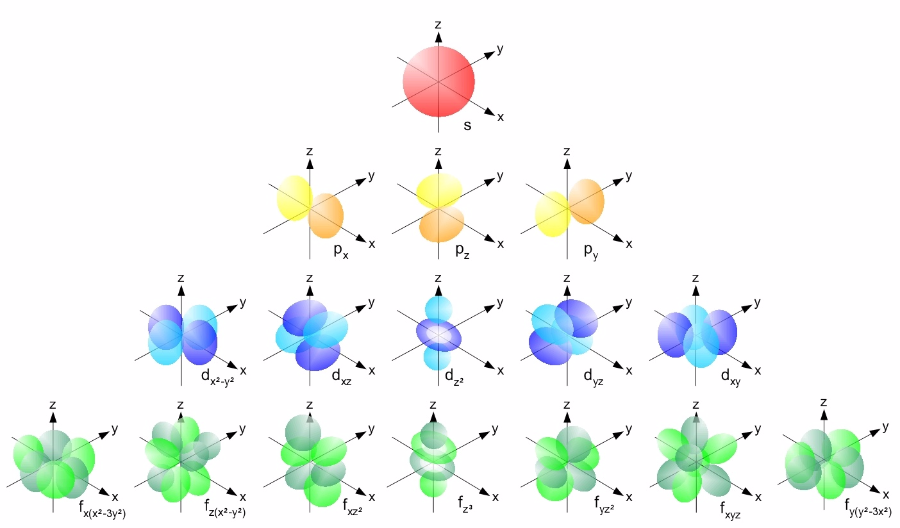
\includegraphics[width=1\linewidth]{Afbeeldingen/orbitalen.png}
    \caption{Typische waarschijnlijkheidsverdelingen voor verschillende golffuncties.}
    \label{fig:orbitalen}
\end{figure}

\section{De Schr\"odingervergelijking}

De vergelijking waarmee de mogelijke golffuncties van een kwantummechanisch systeem worden bepaald, werd in 1926 door Erwin Schr\"odinger voorgesteld. Voor één elektron in één ruimtelijke dimensie en in een toestand met een welbepaalde energie luidt de tijdsonafhankelijke Schr\"odingervergelijking:

\begin{equation}
\boxed{
-\frac{\hbar^2}{2m}
\frac{\partial^2\psi}{\partial x^2}
+
V(x)\psi
=
E\psi,
}
\end{equation}

waarin $\hbar=h/(2\pi)$ de gereduceerde constante van Planck is, $m$ de massa van het elektron, $V(x)$ de potentiële energie en $E$ de totale energie.

De Schr\"odingervergelijking is voor de kwantummechanica wat de bewegingswetten van Newton zijn voor de klassieke mechanica. De vergelijking levert echter niet rechtstreeks de baan of de exacte positie van een elektron. Haar oplossingen zijn de golffuncties die voor het beschouwde systeem mogelijk zijn.

Niet elke willekeurige golffunctie vormt een fysisch aanvaardbare oplossing. De functie moet onder andere eindig, continu en normaliseerbaar zijn. Door deze voorwaarden zijn voor gebonden systemen vaak slechts bepaalde golffuncties en bepaalde energiewaarden toegestaan. De bijbehorende energieën zijn dan gekwantiseerd.

Voor een elektron in een atoom wordt de potentiële energie hoofdzakelijk bepaald door de elektrostatische aantrekking tussen het negatief geladen elektron en de positief geladen kern. De oplossingen van de Schr\"odingervergelijking voor deze potentiële energie leveren de atomaire orbitalen en de bijbehorende energieniveaus.

De stabiliteit van het atoom volgt daarmee niet uit het beeld van een elektron dat in een klassieke baan rond de kern beweegt. Een stabiele atomaire toestand wordt beschreven door een genormaliseerde golffunctie met een welbepaalde energie. De laagste toegelaten oplossing is de grondtoestand. Een toestand waarin het elektron onbeperkt op de kern zou instorten, behoort niet tot de fysisch toegelaten stationaire oplossingen.

\section{Discrete energieniveaus}

Een opmerkelijk gevolg van de Schr\"odingervergelijking is dat slechts een beperkt aantal oplossingen fysisch toegelaten is. Niet elke willekeurige golffunctie voldoet immers aan de randvoorwaarden van het probleem. Alleen golven die op een consistente manier rond de atoomkern kunnen bestaan, blijken stabiele oplossingen te vormen.

Dit kan worden begrepen door een vergelijking te maken met een trillende gitaarsnaar. Wanneer een snaar aan beide uiteinden is vastgemaakt, kan zij niet willekeurig trillen. Slechts bepaalde trillingspatronen zijn mogelijk. Voor de materiegolf van een elektron geldt een gelijkaardig principe: slechts een beperkt aantal golffuncties is mogelijk. Aangezien iedere toegelaten golffunctie overeenkomt met \'e\'en welbepaalde energie, volgt automatisch dat ook slechts een beperkt aantal energieniveaus bestaat.

Zonder bijkomende hypothesen verklaart dezelfde theorie zowel de stabiliteit van atomen als het bestaan van discrete spectraallijnen. Eigenschappen die binnen de klassieke fysica volledig onverklaarbaar bleken, blijken rechtstreeks voort te vloeien uit het golfkarakter van elektronen.

\section{Het waterstofatoom en zijn energieniveaus}

De Schr\"odingervergelijking kan voor het waterstofatoom exact analytisch worden opgelost. De resulterende energieniveaus blijken uitsluitend af te hangen van het hoofdkwantumgetal $n$:
\begin{equation}
E_n = -\frac{13{,}6~\mathrm{eV}}{n^2}, \qquad n = 1,2,3,\ldots
\end{equation}
Hierin is $1~\mathrm{eV} = 1{,}602 \times 10^{-19}~\mathrm{J}$. De negatieve waarde duidt erop dat het elektron aan de kern gebonden is: positieve energie zou een vrij (ongebonden) elektron betekenen.

De laagste energie, de \emph{grondtoestand}, correspondeert met $n=1$ en bedraagt $E_1 = -13{,}6~\mathrm{eV}$. Voor $n=2$ geldt $E_2 = -3{,}4~\mathrm{eV}$, voor $n=3$ geldt $E_3 = -1{,}51~\mathrm{eV}$, enzovoort. Naarmate $n$ groter wordt, nadert de energie aan nul: het elektron wordt steeds zwakker gebonden.

\begin{voorbeeld}{Energie van een foton bij de overgang $n=2 \to n=1$}
Wanneer een waterstofatoom terugvalt van de eerste aangeslagen toestand ($n=2$) naar de grondtoestand ($n=1$), wordt het energieverschil uitgezonden als een foton:
\[
\Delta E = E_2 - E_1 = -3{,}4 - (-13{,}6) = 10{,}2~\mathrm{eV}.
\]
Met $E = h\nu$ en $\lambda = c/\nu$ volgt de golflengte van dit foton:
\[
\lambda = \frac{hc}{\Delta E} = \frac{(6{,}626\times 10^{-34})(2{,}998\times 10^{8})}{(10{,}2)(1{,}602\times 10^{-19})} \approx 1{,}22 \times 10^{-7}~\mathrm{m} = \SI{122}{\nano\meter}.
\]
Dit is de eerste lijn van het Lyman-reeks, in het ultraviolette deel van het spectrum. Deze berekening toont concreet hoe het golfkarakter van het elektron leidt tot discrete spectraallijnen die experimenteel kunnen worden gemeten.
\end{voorbeeld}

\section{Van golffunctie naar chemische energie}

Elke toegelaten oplossing van de Schr\"odingervergelijking wordt gekenmerkt door een welbepaalde golffunctie en een bijbehorende energie. Een elektron kan zich dus niet in een willekeurige energietoestand bevinden, maar uitsluitend in \'e\'en van de discrete energieniveaus die door de vergelijking worden toegelaten.

Hiermee krijgt de chemische energie van een stof een volledig nieuwe betekenis. De energie van een atoom wordt niet bepaald door een klassiek bewogen elektron, maar door de verzameling van kwantummechanisch toegelaten energietoestanden waarin zijn elektronen zich bevinden. Wanneer elektronen tijdens een chemische reactie van energietoestand veranderen, verandert bijgevolg ook de totale energie van het systeem. Chemische energie is dus uiteindelijk een rechtstreeks gevolg van de kwantummechanische energieniveaus van elektronen.

De oplossingen van de Schr\"odingervergelijking worden gekarakteriseerd door hun energie en door de ruimtelijke vorm van hun golffunctie. Iedere oplossing beschrijft een specifieke waarschijnlijkheidsverdeling rondom de atoomkern. Dergelijke oplossingen noemen we \emph{orbitalen}.

Een orbitaal is dus geen bijkomend model dat naast de Schr\"odingervergelijking bestaat. Integendeel, een orbitaal is een oplossing van deze vergelijking. Voor het waterstofatoom kunnen alle oplossingen exact analytisch worden berekend. Het resultaat is een reeks orbitalen die verschillen in energie, grootte en vorm.

De eenvoudigste oplossing van de Schr\"odingervergelijking is de toestand met de laagste energie, de \emph{grondtoestand}. Voor het waterstofatoom komt deze overeen met het zogenaamde 1s-orbitaal. De waarschijnlijkheidsverdeling is volledig bolsymmetrisch: de kans is het grootst dicht bij de kern en neemt geleidelijk af naarmate de afstand groter wordt.

Wanneer meerdere oplossingen van de Schr\"odingervergelijking bestaan, moeten we deze op een ondubbelzinnige manier kunnen onderscheiden. Elke toegelaten golffunctie wordt volledig bepaald door vier \emph{kwantumgetallen}:

\begin{itemize}
\item Het \emph{hoofdkwantumgetal} $n$ bepaalt in de eerste plaats de energie van het elektron en geeft een indicatie van de gemiddelde afstand tot de atoomkern.
\item Het \emph{azimutaal kwantumgetal} $l$ bepaalt de vorm van het orbitaal. Hieruit volgen de bekende $s$-, $p$-, $d$- en $f$-orbitalen.
\item Het \emph{magnetisch kwantumgetal} $m_l$ beschrijft de ruimtelijke ori\"entatie van een orbitaal.
\item De \emph{spin} $m_s$ kan slechts twee waarden aannemen, $+\tfrac{1}{2}$ en $-\tfrac{1}{2}$. Hoewel de naam doet vermoeden dat een elektron om zijn eigen as draait, is dit beeld slechts een analogie. Spin is een fundamentele kwantummechanische eigenschap zonder klassiek equivalent.
\end{itemize}

Een golffunctie moet overal in de ruimte een continue en fysisch aanvaardbare oplossing vormen van de Schr\"odingervergelijking. Hierdoor zijn slechts bepaalde ruimtelijke golfpatronen mogelijk, net zoals een trillende snaar slechts bepaalde staande golven kan aannemen.

Bij een staande golf op een snaar zijn er plaatsen die nooit bewegen. Deze punten worden \emph{knopen} genoemd. Op analoge wijze bestaan er in een atoom oppervlakken waarop de golffunctie precies nul is. Deze worden \emph{knoopoppervlakken} genoemd. Omdat de waarschijnlijkheidsdichtheid wordt gegeven door $|\psi|^2$, is de kans om een elektron op een knoopoppervlak aan te treffen exact nul.

Het eenvoudigste golfpatroon bezit geen knoopoppervlakken en komt overeen met het bolsymmetrische $1s$-orbitaal. Hogere oplossingen van de Schr\"odingervergelijking bevatten één of meerdere knoopoppervlakken, waardoor de golffunctie afwisselend positieve en negatieve waarden aanneemt. Hoewel deze tekenverandering geen invloed heeft op de waarschijnlijkheidsdichtheid - $|\psi|^2$ is immers steeds positief - bepaalt zij wel de vorm van het orbitaal en de manier waarop verschillende golffuncties met elkaar kunnen interfereren.

Iedere bijkomende knoop betekent dat de golffunctie sterker moet variëren in de ruimte. Wiskundig komt dit overeen met een grotere kromming van de golffunctie, waardoor de kinetische energie van het elektron toeneemt. De kromming van de golffunctie is namelijk een maat voor de kinetische energie  van het elektron op die plaats. Orbitalen met meer knoopoppervlakken bezitten daarom automatisch een hogere totale energie dan orbitalen met minder knopen.

Dit is volledig analoog aan een trillende gitaarsnaar. De grondtoon bezit geen inwendige knopen en heeft de laagste energie. Hogere boventonen bevatten steeds meer knopen en vereisen een hogere trillingsenergie. Op dezelfde manier beschrijven de verschillende atomaire orbitalen de toegelaten staande golven van de elektrongolffunctie. Meer knoopoppervlakken komen overeen met hogere energietoestanden.

\section{Het uitsluitingsprincipe van Pauli}

De Schr\"odingervergelijking levert de toegelaten orbitalen waarin elektronen zich kunnen bevinden. Daarmee is echter nog niet bepaald hoe meerdere elektronen over deze orbitalen worden verdeeld. De ontbrekende bouwsteen werd in 1925 geleverd door Wolfgang Pauli.

Pauli formuleerde het \emph{uitsluitingsprincipe}, dat stelt dat twee elektronen binnen hetzelfde atoom nooit volledig dezelfde kwantumtoestand kunnen bezitten. Anders geformuleerd: geen twee elektronen mogen dezelfde vier kwantumgetallen hebben.

\begin{definitie}{Uitsluitingsprincipe van Pauli}
Elk orbitaal kan maximaal twee elektronen bevatten. Wanneer twee elektronen hetzelfde orbitaal bezetten, moeten zij een tegengestelde spin hebben. Het uitsluitingsprincipe is geen gevolg van de elektrostatische afstoting tussen elektronen, maar een fundamentele eigenschap van de natuur die geldt voor alle fermionen.
\end{definitie}

Een orbitaal wordt immers volledig beschreven door de drie kwantumgetallen die de vorm en oriëntatie bepalen. Indien twee elektronen hetzelfde orbitaal bezetten, verschillen zij enkel nog in hun vierde kwantumgetal: de spin. Daarom kan een orbitaal slechts twee elektronen bevatten, één met spin $+\tfrac{1}{2}$ en één met spin $-\tfrac{1}{2}$. De reden hiervoor ligt diep verankerd in de kwantummechanica. Elektronen zijn \emph{fermionen} en worden beschreven door een antisymmetrische golffunctie. Wanneer twee elektronen dezelfde vier kwantumgetallen zouden bezitten, zou deze gezamenlijke golffunctie overal nul worden. Een dergelijke toestand is fysisch onmogelijk, waardoor twee elektronen nooit volledig dezelfde kwantumtoestand kunnen innemen.

Het uitsluitingsprincipe heeft ingrijpende gevolgen voor de opbouw van atomen. Zodra een orbitaal door twee elektronen is bezet, moeten bijkomende elektronen uitwijken naar een orbitaal met een hogere energie. Hierdoor ontstaat automatisch een gelaagde elektronenstructuur met schillen en subschillen.

Een goede analogie is een gebouw met appartementen. Elk appartement stelt een orbitaal voor en biedt slechts plaats aan twee bewoners. Zodra een appartement volledig bezet is, moeten nieuwe bewoners verhuizen naar een appartement op een hogere verdieping. Op analoge wijze worden de orbitalen in een atoom geleidelijk opgevuld volgens toenemende energie.

Vanuit chemisch oogpunt is dit een van de belangrijkste resultaten van de kwantummechanica. De Schr\"odingervergelijking bepaalt welke orbitalen bestaan en welke energie zij bezitten, terwijl het uitsluitingsprincipe van Pauli vastlegt hoe deze orbitalen worden opgevuld. Samen verklaren zij de elektronenconfiguraties van alle elementen en vormen zij de basis voor het periodiek systeem, de chemische binding en uiteindelijk de enorme verscheidenheid aan chemische stoffen.

\section{Van kwantummechanica naar het periodiek systeem}

Met de Schr\"odingervergelijking kunnen de toegelaten orbitalen en hun energieniveaus worden berekend. Het uitsluitingsprincipe van Pauli bepaalt vervolgens hoeveel elektronen ieder orbitaal maximaal kan bevatten. Samen verklaren deze principes hoe de elektronenconfiguratie van een atoom ontstaat.

Bij het opbouwen van een atoom worden de elektronen niet willekeurig verdeeld. Zij bezetten eerst de orbitalen met de laagste energie. Dit staat bekend als het \emph{Aufbauprincipe}, afgeleid van het Duitse woord \emph{Aufbau}, dat ``opbouw'' betekent.

Wanneer meerdere orbitalen dezelfde energie bezitten, zoals de drie $p$-orbitalen of de vijf $d$-orbitalen, geldt bovendien de \emph{regel van Hund}. Elektronen vullen deze orbitalen eerst afzonderlijk op, telkens met een gelijke spin, voordat een tweede elektron aan een reeds bezet orbitaal wordt toegevoegd. Op die manier wordt de totale energie van het atoom zo laag mogelijk gehouden.

De opbouw van de eerste elementen illustreert deze regels:

\begin{align*}
\text{H:}  &\qquad 1s^1 \\
\text{He:} &\qquad 1s^2 \\
\text{Li:} &\qquad 1s^2\,2s^1 \\
\text{Be:} &\qquad 1s^2\,2s^2 \\
\text{B:}  &\qquad 1s^2\,2s^2\,2p^1_x \\
\text{C:}  &\qquad 1s^2\,2s^2\,2p^1_x\, 2p^1_y \\
\text{N:}  &\qquad 1s^2\,2s^2\,2p^1_x\,2p^1_y\,2p^1_z \\
\text{O:}  &\qquad 1s^2\,2s^2\,2p^2_x\,2p^1_y\,2p^1_z \\
\end{align*}

Voor stikstof worden de drie elektronen in de $2p$-schil eerst verdeeld over drie verschillende orbitalen. Pas vanaf zuurstof begint de vorming van elektronenparen in de $2p$-orbitalen.

De volgorde waarin de orbitalen worden opgevuld wordt bepaald door hun energie. Voor de meeste elementen geldt de volgende opvulvolgorde:

\begin{equation*}
1s
\rightarrow
2s
\rightarrow
2p
\rightarrow
3s
\rightarrow
3p
\rightarrow
4s
\rightarrow
3d
\rightarrow
4p
\rightarrow
5s
\rightarrow
4d
\rightarrow
5p
\rightarrow
6s
\rightarrow
4f
\rightarrow
5d
\rightarrow
\cdots
\end{equation*}

Hoewel deze volgorde op het eerste gezicht verrassend lijkt, volgt zij rechtstreeks uit de oplossingen van de Schr\"odingervergelijking. De energie van een orbitaal wordt niet uitsluitend bepaald door de afstand tot de kern, maar ook door de vorm van de golffunctie en de afscherming door andere elektronen. Hierdoor ligt het $4s$-orbitaal bijvoorbeeld iets lager in energie dan de $3d$-orbitalen en wordt het doorgaans eerst opgevuld.

De elektronen in de buitenste schil, de \emph{valentie-elektronen}, bepalen in grote mate de chemische eigenschappen van een element. Elementen met eenzelfde aantal valentie-elektronen vertonen daarom vergelijkbaar chemisch gedrag en komen in dezelfde groep van het periodiek systeem terecht.

Het periodiek systeem is daardoor geen toevallige ordening van elementen, maar een rechtstreeks gevolg van de wetten van de kwantummechanica. De Schr\"odingervergelijking bepaalt de toegelaten orbitalen, het uitsluitingsprincipe van Pauli legt vast hoeveel elektronen elk orbitaal kan bevatten, het Aufbauprincipe beschrijft de volgorde waarin de orbitalen worden opgevuld en de regel van Hund bepaalt hoe elektronen over gelijkwaardige orbitalen worden verdeeld. Samen verklaren deze principes de elektronenconfiguraties van alle elementen en vormen zij de basis van de chemische binding, de molecuulstructuur en uiteindelijk de enorme verscheidenheid aan stoffen die in de natuur voorkomen.

Daarmee vormt de kwantummechanica de brug tussen de fundamentele natuurkunde van het atoom en de chemie van materialen, reacties en processen. Wat begon als een zoektocht naar de verklaring van het gedrag van licht en elektronen, mondt uit in een theorie die de volledige opbouw van het periodiek systeem en daarmee een groot deel van de chemie verklaart.

\section{De vorming van chemische bindingen}

Wanneer twee atomen dicht genoeg naar elkaar worden gebracht, beginnen hun golffuncties elkaar te be\"invloeden. Op dat ogenblik ontstaat een \emph{chemische binding}. Het is fundamenteel om te begrijpen dat een binding niet ontstaat doordat de atomen simpelweg aan elkaar ``kleven'', maar doordat hun gemeenschappelijke golffunctie een nieuwe, stabiele oplossing vormt van de Schr\"odingervergelijking.

Een chemische binding vormt omdat het samengebrachte systeem een lagere energie kan bereiken dan de gescheiden atomen afzonderlijk. De totale energie wordt bepaald door de nieuwe gemeenschappelijke golffunctie. Wanneer deze een energetisch gunstiger configuratie oplevert, ontstaat spontaan een binding.

\section{Constructieve en destructieve interferentie}

Wanneer twee golffuncties worden samengebracht, kan dit op twee manieren gebeuren. Wanneer de golffuncties in fase zijn, versterken zij elkaar: dit heet \emph{constructieve interferentie} en leidt tot een bindende toestand met lagere energie. Wanneer de golffuncties in tegenfase zijn, heffen zij elkaar op: dit heet \emph{destructieve interferentie} en leidt tot een antibindende toestand met hogere energie.

\section{Bindingsenergie en reactie-enthalpie}

Uit de combinatie van bindende en antibindende orbitalen ontstaat het fundamentele inzicht dat chemische energie niets anders is dan het energieverschil tussen de elektronenconfiguratie van de reagentia en deze van de reactieproducten. Bij de vorming van een chemische binding bereiken de elektronen een lagere energietoestand; het energieverschil wordt vrijgesteld.

Wanneer tijdens een chemische reactie bestaande bindingen worden verbroken en nieuwe bindingen worden gevormd, verandert de totale energie van het systeem. Het verschil tussen de bindingsenergie\"en van de reagentia en deze van de reactieproducten bepaalt de \emph{reactie-enthalpie}. Een negatieve reactie-enthalpie betekent dat de producten energetisch gunstiger zijn dan de reagentia: warmte wordt vrijgesteld. Een positieve reactie-enthalpie betekent dat het systeem energie moet opnemen.

Hiermee wordt de brug geslagen tussen de kwantummechanische beschrijving van individuele elektronen en de macroscopische thermodynamica. De enthalpie die in het vorige hoofdstuk werd ingevoerd, vindt haar uiteindelijke oorsprong in de kwantummechanische energietoestanden van elektronen.

\section{Bindingslengte en evenwicht}

Wanneer twee atomen te ver van elkaar verwijderd zijn, is hun golffunctie-overlap te klein om een binding te vormen. Wanneer zij te dicht bij elkaar worden, stijgt de energie door de afstoting tussen de kernen. Op een welbepaalde afstand is de totale energie minimaal: dit is de \emph{evenwichtsafstand} of \emph{bindingslengte}. De welbepaalde lengte van een chemische binding is dus een rechtstreeks gevolg van het evenwicht tussen aantrekkelijke en afstotende krachten op atomaire schaal.

\section{Kinetische beperkingen op spontane reacties}

Wanneer een systeem een lagere energietoestand kan bereiken door nieuwe bindingen te vormen, zou men verwachten dat deze omzetting spontaan en onmiddellijk verloopt. De werkelijkheid blijkt echter veel complexer. Diamant is bij kamertemperatuur thermodynamisch minder stabiel dan grafiet, maar een diamant verandert niet spontaan in een klomp grafiet. Een mengsel van waterstof en zuurstof bezit voldoende energie om explosief tot water te reageren, maar kan jarenlang onveranderd worden bewaard.

Blijkbaar is een lagere energie alleen niet voldoend om een reactie spontaan te laten verlopen. Naast de energie van begin- en eindtoestand moeten we ook de weg bekijken die het systeem tussen beide toestanden moet afleggen.

\section{Activeringsenergie en overgangstoestand}

Tijdens een chemische reactie verdwijnen oude bindingen niet op hetzelfde ogenblik waarop nieuwe bindingen ontstaan. De elektronenwolk moet zich voortdurend aanpassen terwijl atomen dichter bij elkaar komen, bestaande bindingen worden uitgerekt en nieuwe bindingen geleidelijk ontstaan. Gedurende dit proces bevindt het systeem zich in een opeenvolging van tijdelijke elektronenconfiguraties. Sommige hiervan zijn energetisch minder gunstig dan zowel de reagentia als de reactieproducten.

De minimale energie die nodig is om deze \emph{overgangstoestand} te bereiken, noemen we de \emph{activeringsenergie}. Het bestaan van een activeringsenergie verklaart waarom een reactie tegelijkertijd thermodynamisch gunstig en kinetisch traag kan zijn. De thermodynamica bepaalt welke toestand uiteindelijk het stabielst is, terwijl de kinetiek bepaalt hoe snel het systeem deze toestand kan bereiken.

\begin{besluit}{Van kwantummechanica naar thermodynamica}
De enthalpie van een systeem weerspiegelt uiteindelijk de energie die besloten ligt in de chemische bindingen, en dus in de kwantummechanische energietoestanden van de elektronen. De entropie, die we in het volgende hoofdstuk zullen introduceren, beschrijft daarentegen het aantal verschillende manieren waarop energie en materie over het systeem kunnen worden verdeeld. Beide bijdragen worden samengebracht in de Gibbs-vrije energie $G = H - TS$. De kwantummechanica en de thermodynamica blijken daarmee geen afzonderlijke theorie\"en te zijn, maar twee complementaire beschrijvingen van hetzelfde fysische systeem.
\end{besluit}
